%%%%%%%%%%%%%%%%%%%%%%%%%%%%%%%%%%%%%%%%%
%%% WP01
%%%%%%%%%%%%%%%%%%%%%%%%%%%%%%%%%%%%%%%%%

\tsubsubsection{WP03 - Access to RI for Accelerators}

%%%%%%%%%%%%%%%%%%%%%%%%%%%%%%%%%%%%%%%%%
%%% Section content, please change!
%%%%%%%%%%%%%%%%%%%%%%%%%%%%%%%%%%%%%%%%%

\subsubsection*{Overview and Goals}

\begin{table}[H]
    \renewcommand{\arraystretch}{1.50}		
    \footnotesize   
    \begin{tabular}{*{3}{|p{0.10\textwidth}}|l|}
        \hline
        \rowcolor{mygray} \multicolumn{4}{|c|}{\textit{\color{white}Work Package Summary}} \\
        \hline
        \rowcolor{mylightergray} \textit{WP No.} & \cellcolor{white} 01 & \textit{Title of WP} & \cellcolor{white} WP Title \\
        \hline
        \rowcolor{mylightergray} \textit{Start} & \cellcolor{white} Mxx & \textit{End} & \cellcolor{white} Myy \\
        \hline
        \rowcolor{mylightergray} \multicolumn{4}{|p{0.978\textwidth}|}{\textit{Participating Organisations}} \\
        \hline
        \multicolumn{4}{|p{0.978\textwidth}|}{
            \hspace*{-0.75cm} 
            \begin{minipage}[t]{\textwidth}
    			\begin{itemize}
    			    \item WP Leader: Partner 1
    				\item Participants: Partner 2, Partner 3, Partner 4, Partner 5, Partner 6, Partner 7
    			\end{itemize} 
    			\vspace*{0.10em}
			\end{minipage}
        } \\
        \hline
    \end{tabular}
    \vspace{0.5em}\vfill
    \begin{tabular}{|p{0.978\textwidth}|}
        \hline
        \rowcolor{mylightergray} \textit{Goals} \\
        \hline
        \rowcolor{white} 
        \hspace*{-0.75cm} 
        \begin{minipage}[t]{\textwidth}
    		\begin{itemize}
    		    \item Goal 1
    			\item Goal 2
			    \item Goal 3
    		\end{itemize} 
    		\vspace*{0.10em}
		\end{minipage}        
        \\
        \hline
    \end{tabular}
    \vspace{0.5em}\vfill
    \begin{tabular}{|l|*{7}{>{\centering\arraybackslash}p{0.084\textwidth}|}}
        \hline    
        \rowcolor{mylightergray} \textit{Participant number} & \textit{1} & \textit{2} & \textit{3} & \textit{4} & \textit{5} & \textit{6} & \textit{7} \\
        \hline
        \rowcolor{white} \cellcolor{mylightergray}\textit{Participant short name} & Partner 1 & Partner 2 & Partner 3 & Partner 4 & Partner 5 & Partner 6 & Partner 7 \\
        \hline
        \rowcolor{white} \cellcolor{mylightergray}\textit{PM per participant} & xx & xx & xx & xx & xx & xx & xx \\
        \hline        
    \end{tabular}    
\end{table}

\subsubsection*{Status}

\todo{Briefly explain the status of the WP.}

\subsubsection*{Progress per Task}

\subparagraph{Task 3.1 Material Testing Facilities} \mbox{}

This task includes the High-Radiation to Materials (HiRadMat) Faclity at CERN. 

HiRadmat has had great progress in the last reference period concerning EURO-LABS. The facility remains in extremely high demand from the international community, involving both EU and overseas teams that are performing experiments. A total of 3928 AUs have been spend (from the total requested 4800). The percentage of AUs spent vs the available AUs are shown in Figure~\ref{fig:stat_pie_hiradmat}. Given the high demand for the facility also in view of the CERN's long shutdown between 2026-2029, HiRadMat could welcome also more access units in case they become available, in order to support the experiments in 2026. 

\begin{figure}[!h]
    \centering
    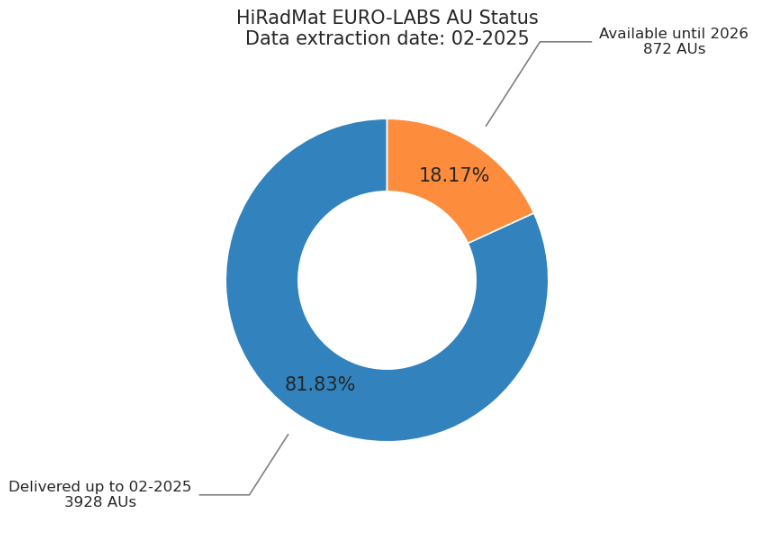
\includegraphics[width=0.75\linewidth]{graphics/stat_pie_hiradmat.png}
    \caption{Access Units spent in HiRadMat in all reference periods. A total of 4800 AUs were allocated in total ; 3696 AUs have been already spent in this second reference period, and 232 AUs have been spent after September 2024 and until today (Feb. 2025). }
    \label{fig:stat_pie_hiradmat}
\end{figure}

For the funded users, the gender distribution is shown also in Figure~\ref{fig:gender_distr_hiradmat}, removing the duplicates by name. 

\begin{figure}[!h]
    \centering
    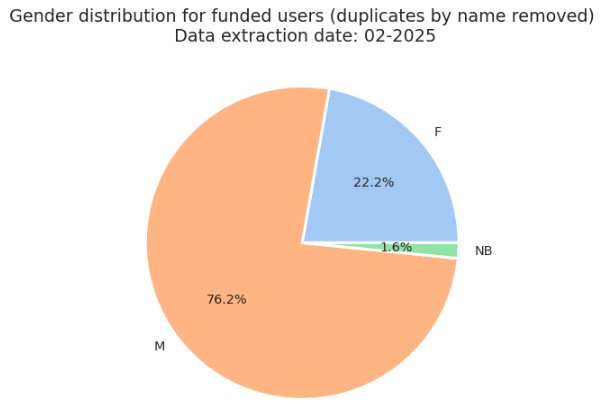
\includegraphics[width=0.6\linewidth]{graphics/gender_distr_hiradmat.png}
    \caption{Gender distribution of TA funded users for Task Force 3.1 (HiRadMat)}
    \label{fig:gender_distr_hiradmat}
\end{figure}

The age distribution of the funded users, is indicating that as per the instructions for TA, the user selection panel has approved mostly undergraduate and postgraduate students, at the early stages of their careers and fewer senior researchers (professors and tenured researchers). However, specifically at HiRadMat, the presence of the senior persons in the preparatory, data-taking and experimental phases is absolutely necessary for the success of the experiments. The age distribution for the funded users is shown in Figure~\ref{fig:age_distr_hiradmat}.

\begin{figure}[!h]
    \centering
    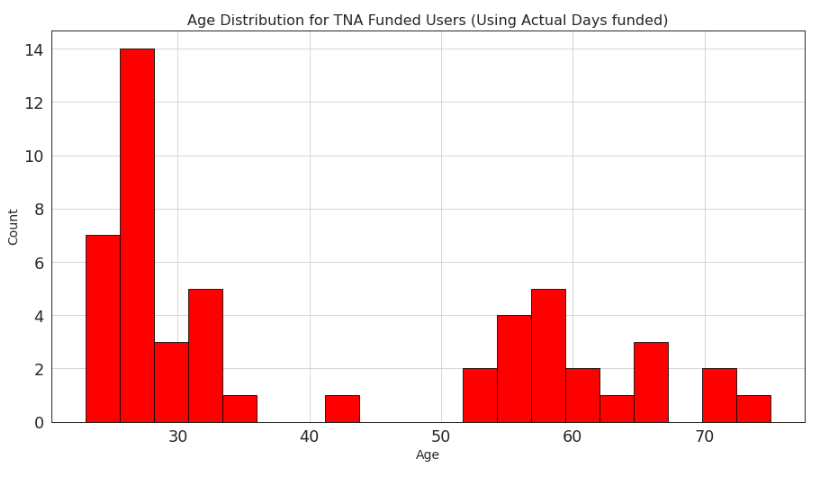
\includegraphics[width=0.75\linewidth]{graphics/age_distr_hiradmat.png}
    \caption{Age distribution of funded users in Task 3.1 (HiRadMat). The majority of the supported users is at the early stages of their career, while a few senior researchers or recognized scientists at their field have been also necessary during the preparatory or the post-irradiation phases.}
    \label{fig:age_distr_hiradmat}
\end{figure}

The evolution of the spent access units overall, and only for the RP2 is shown in Figures~\ref{fig:overall_evolution_hiradmat} and~\ref{fig:RP2_evolution_hiradmat}.

\begin{figure}[!h]
    \centering
    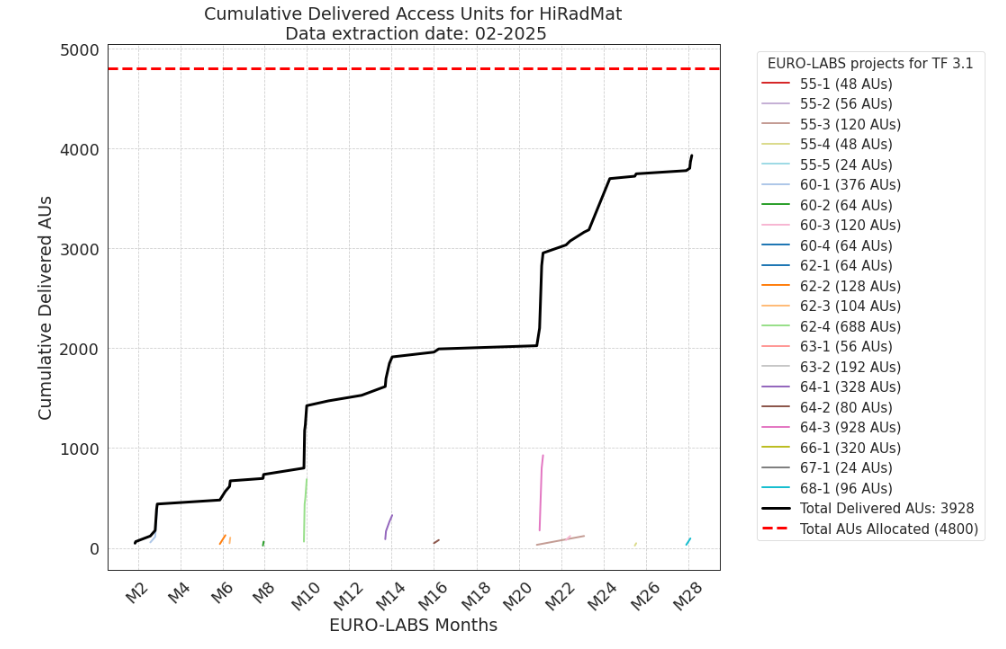
\includegraphics[width=0.9\linewidth]{graphics/overall_evolution_hiradmat.png}
    \caption{Overall evolution of delivered AUs for HiRadMat and breakdown of AUs per project.}
    \label{fig:overall_evolution_hiradmat}
\end{figure}

\begin{figure}[!h]
    \centering
    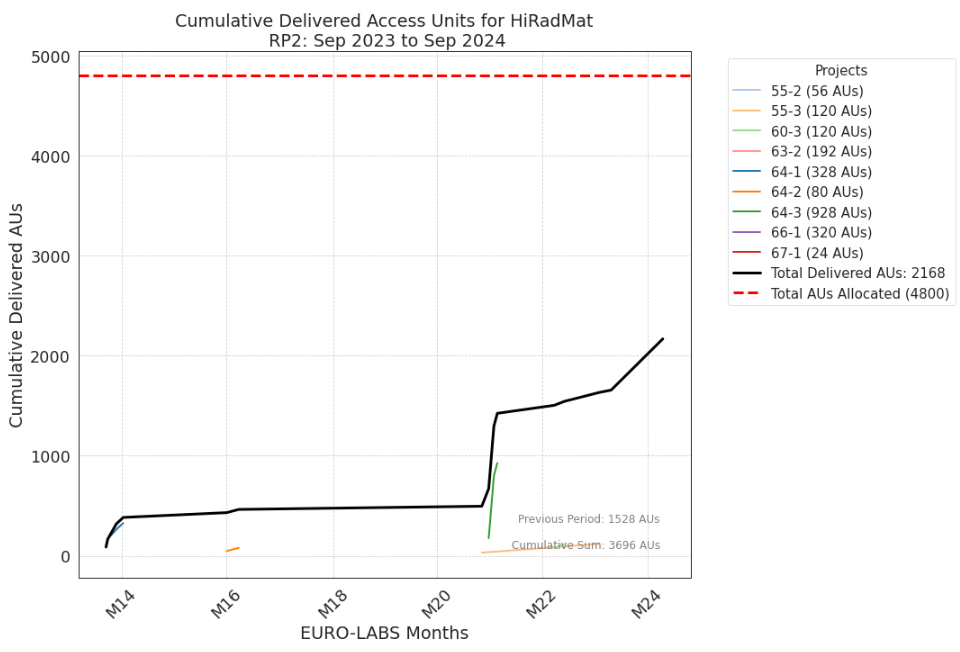
\includegraphics[width=0.9\linewidth]{graphics/RP2_evolution_hiradmat.png}
    \caption{Evolution of delivered AUs for HiRadMat during the second reference period (RP2) and breakdown of AUs per project.}
    \label{fig:RP2_evolution_hiradmat}
\end{figure}

\subsubsection*{Main Results and Achievements}

Many of the HiRadMat experiments produced great results during this second reference period. The results of the \textbf{HRMT-62} and \textbf{HRMT-64} experiments have an extremely high impact. In particular, up to-date, 5 peer-reviewed articles have been written, 3 of them published in or submitted to Nature, all citing the EURO-LAB support. In total, 14 press releases have been done by the collaborating institutes, including 2 from CERN (bulletin \& courrier). It worth noting that the articles have a high ``attention score'', of 260: 99th percentile of the 329,972 tracked articles of a similar age in all journals. The key scientific result from HRMT-64, only made possible with the EURO-LABS support, was the first-time measurement of the magnetic fields produced by plasma instabilities using a Faraday rotation, seen in Figure~\ref{fig:hiradmat_mag_field_plasma}.

\begin{figure}[!h]
    \centering
    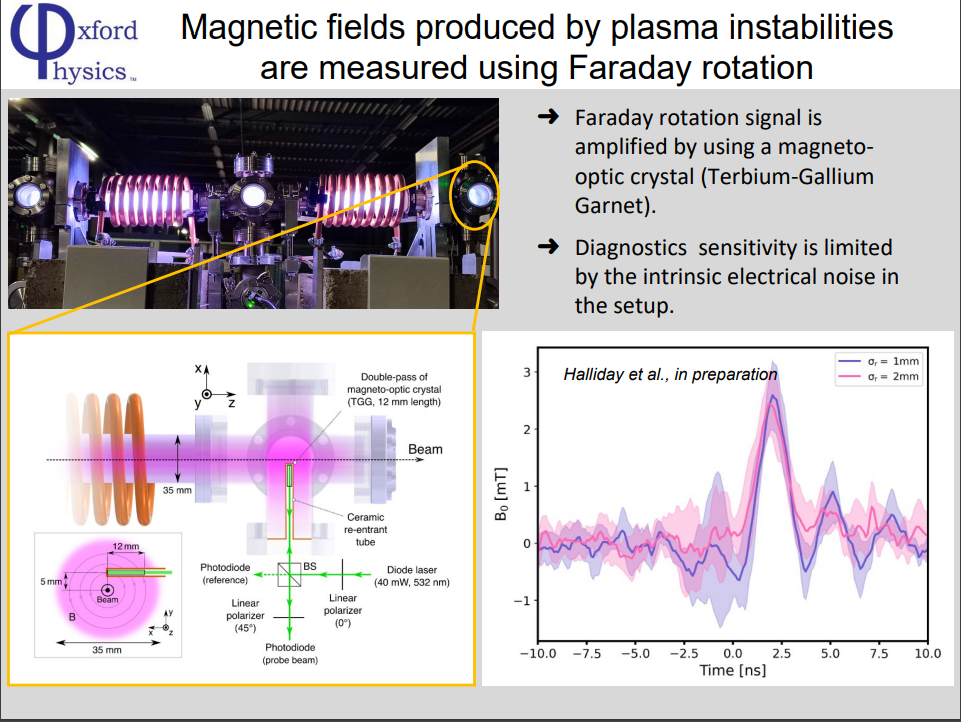
\includegraphics[width=0.75\linewidth]{graphics/HRMT_64_magnetic_field.png}
    \caption{HRMT-64, with the EURO-LABS support measured for first time the magnetic fields produced by plasma instabilities using a faraday rotation in HiRadMat. Courtesy: Prof. G. Gregori, Univ. of Oxford.}
    \label{fig:hiradmat_mag_field_plasma}
\end{figure}

\textbf{HRMT-66} was a novel experiment that pushed forward our current knowledge of material limits, particularly for the often used Glassy Carbon and Beryllium, along with a first-time irradiation of Si$_{3}$N$_{4}$ in order to investigate its exact damage threshold. This is very important for the cooling section of a future muon collider. A photo from the results is shown in Figure~\ref{fig:hiradmat_Si3N4} for Si$_{3}$N$_{4}$ and in Figure~\ref{fig:hiradmat_GC} for Glassy Carbon. 

\begin{figure}[!h]
    \centering
    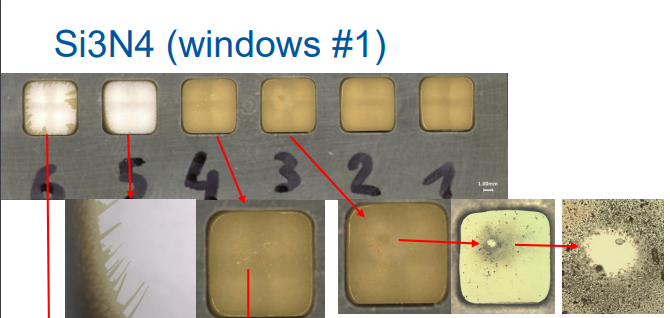
\includegraphics[width=0.75\linewidth]{graphics/hiradmat_si3n4.png}
    \caption{Beam impact on Si3N4 windows during HRMT-66 experiment. The support of EURO-LABS was extremely important since FLUKA simulations were absolutely necessary for the evaluation of the damage mechanisms and precence at CERN was vital for some of the collaborators of the experiment.(Courtesy: A. Harrison, CERN)}
    \label{fig:hiradmat_Si3N4}
\end{figure}

\begin{figure}[!h]
    \centering
    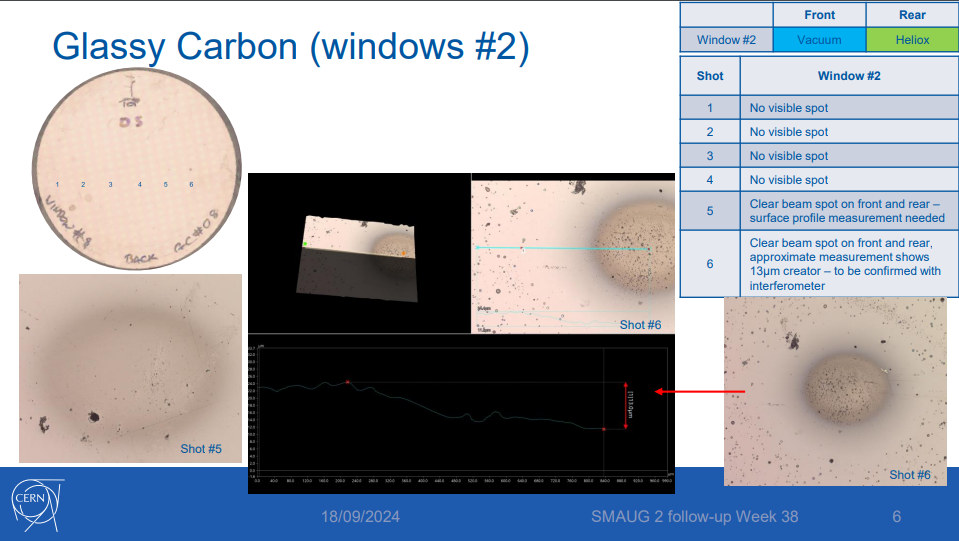
\includegraphics[width=0.75\linewidth]{graphics/hiradmat_GC.png}
    \caption{Results from HRMT-66 experiment on Glassy Carbon. The clearb beam spot can be seen in shot \#6 including a small crater.}
    \label{fig:hiradmat_GC}
\end{figure}

\textbf{HRMT-55} concluded in 2024, and a follow-up experiment, \textbf{HRMT-71}
is planned to take place in 2025. This is a collaboration between CERN and ESS, with the results being useful for both organisations.

The results indicate similar detector performance for all ionisation chambers (IC), however detector to detector performance differences were observed. See for example Figure~\ref{fig:hiradmat_IC_response}. In order to complete documentation and validate future designs, \textbf{HRMT-71} will also request funding from EURO-LABS, in particular for the ESS relevant part. 

\begin{figure}[!h]
    \centering
    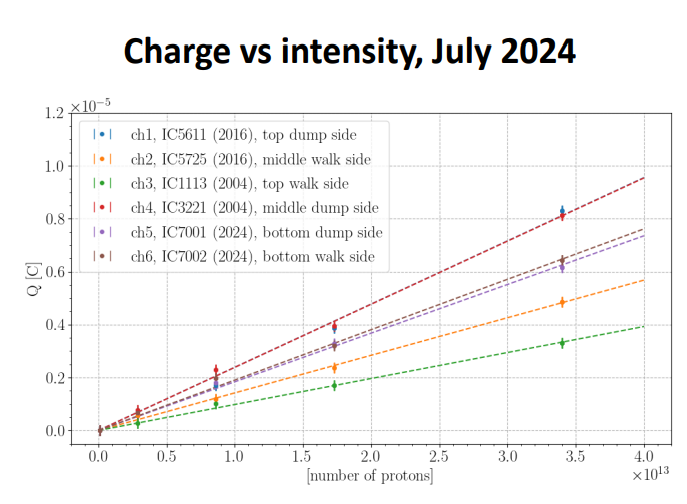
\includegraphics[width=0.8\linewidth]{graphics/hiradmat_IC_response.png}
    \caption{Response (C) of the different ionization chambers tested in HRMT-55. The difference in the slope needs to be understood in detail in a follow-up experiment (HRMT-71) planned for 2025. (Courtesy. S. Grishin, ESS)}
    \label{fig:hiradmat_IC_response}
\end{figure}

\subsubsection*{Progress in the service improvements tasks assigned for HiRadMat}

EURO-LABS is supporting a service improvement part for HiRadMat that is focused on improving the calibration of the SPS Beam Position Monitor System (designated ``ALPS'), that also affects HiRadMat. The beam position precision, in particular for experiments like HRMT-62 and HRMT-64 is very important, and for the moment is not fully reliable. 

As part of this task, a neural network is being developed that would improve the residual errors for the device calibration, that today is done via a simple polynomial fit. 

The task is quite complicated and with ambiguous results : The performance of the existing calibration curve was never studied in this way before. This task is well ongoing (via a doctoral student that works at CERN in collaboration with Univ. of Oxford). 

It needs to be noted that the algorithm of choice will be developed by the end of 2025 and a report will be written by then. However \textbf{no implementation can happen before 2029}, i.e after the CERN long shutdown. This aligns with the timeline and the schedule for this particular task of the project, since it will allow proper prototyping and testing of the new electronic components during the CERN long shutdown between 2026-2029. 

First preliminary results comparing the residuals produced by a neural network vs the old polynomial fit approach, taking into account the response of a single electrode of an ALPS Beam Position Monitor (BPM), can be seen in Figure~\ref{fig:hiradmat_SI}. Further optimization studies towards the minimization of errors in terms of beam position measurements are ongoing.
\begin{figure}[!h]
    \centering
    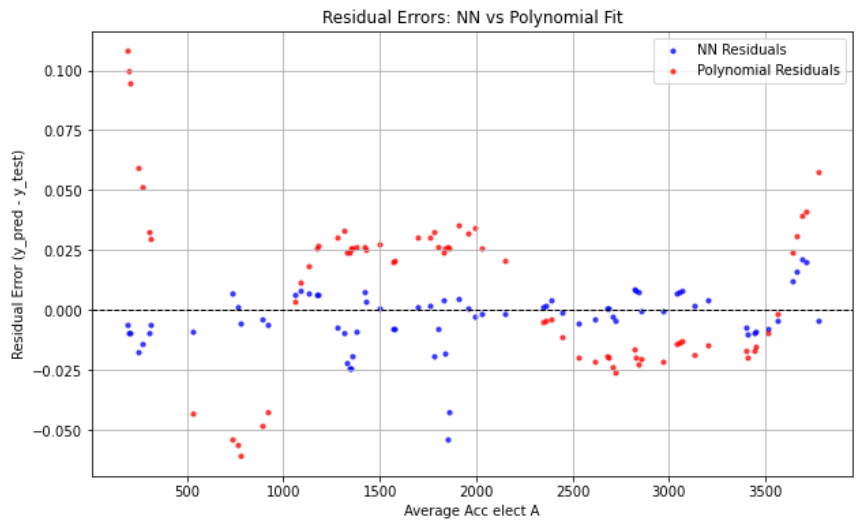
\includegraphics[width=0.75\linewidth]{graphics/hiradmat_SI.png}
    \caption{Residuals for the calibration curve of an ALPS beam position monitor, for the response of a single electrode. The newly developed neural network seems to outperform the old polynomial fit. (Courtesy, V. Stergiou, A. Boccardi (CERN)).}
    \label{fig:hiradmat_SI}
\end{figure}

\subsubsection*{Deviations and Corrective Actions}

HiRadMat has spent in the second reference period already 82\% of the 4800 allocated AUs. This is due to the facility's publicity (also thanks to EURO-LABS dissemination efforts and the promotional videos). The AUs left can cover a part of the 2025 experiments, however there will be no budget left to support the rest of the 2025 and the 2026 experiments (the number of which is, currently uncertain). Therefore, in case that other facilities will not manage to spend, HiRadMat would welcome some additional funding for TA and for support to the users with logistics and simulations. 


\subparagraph{Task 3.2 : Technology Infrastructures} \mbox{}

\todo{Briefly explain the progress of the task in context to the DoA.}

\subsubsection*{Main Results and Achievements}

\subparagraph{UU-FREIA}

Despite the promising startup in P1, FREIA has not provided any TA during this period. There were some brief discussions about testing a PIP II cavity, but unfortunately there has been no follow up.

 
%To answer your questions/s: yes, they are interested in using our facility and will sign the document (it’s already done by our side), but you know how it is with especially MYRRHA, we are requested to not give any information (let it be slides, or just in a general chat) if it has not been previously approved by them. And even more without a signed contract…So unfortunately this is not just because we do not have yet have a signed contract, this will always be the case: they being mention in any way in future slides will need to be sent for their approval.
 

% I write you because we are in initial discussions with FNAL about the possibility of testing a PIPII cavity in Gersemi, and I have a question that I forgot the answer to after the SAM…Provided the TA is granted by the committee, the total amount of units that FREIA can provide, is it the 20\% of the total? For example, FREIA has a total of 960 TA units, could we then only provide max 192 TA units for this test? So could they then pay the rest of the amount themselves if needed?

% Since we do not know how is it going to look in the future for us (since we will have the liquefier kind of blocked by Minerva testing, with some small slots here and there, maybe) we would like to have this test done and accounted, even though it is not from an European Institution.


\subparagraph{INFN-LASA}


LASA is characterized by the presence of four test facilities devoted to:
•	Superconducting (SC) Magnets
•	Superconducting (SC) RF Cavities
•	High Brightness Photocathodes for Electron Sources
•	Laser Applications to High Power Fabry Perot Cavities and Advanced Timing Systems.

The four facilities have been conceived at the beginning as research facilities for the activities undergoing at LASA.

The activities relating to a transition of these facilities towards use by external users slowed down during 2023 compared to the initial projects for two reasons:
the commitment of a relevant part of the researchers involved and of the technical support (the latter already quite limited) of the laboratory in relation to the planning of the expansion of the LASA (by a factor equal to approximately 100% of the surface)
the design of the new infrastructures relating to the electrical systems and the cavity and magnet cooling system of the current laboratory.

Once these activities have been completed, we are now able to prepare the forwarding of requests discussed and received in the meantime in relation to some specific activities.
Of course due to the specific period of the year we have to discuss the confirmation for these previous requests. 

Superconducting cavities: we discussed a request from researchers from DESY and CEA for the test of a prototype SC RF cavity for the PIP II project. The test will last a week considering 3 days for cooling down and one for warming up. The measurement process will last 2 days (for a total of nearly 12 hours/each day to save on liquid helium). Looking at the relatively short time dedicated to the measurements we are evaluating the possibility to operate in a remote fashion.
The same opportunity for a separate test with longer measurements time involved will be used by a researcher from JLab to learn as much as possible on handling SC RF cavities for an ERL Linac of mutual interest. For this request we have to consider also some issue related to the availability of the requested volume of liquid helium (1500 liters) with so a short forewarning.

Laser applications: a request has been discussed about a user from IJCLab and University of Orsay to carry out measurements on the laser system available at LASA for photocathode and Fabry Perot cavity. He plans to stay here a week (5 days) working 8-10 hours every day. This would be the first activity of a longer usage of our facility.

High Brightness Photocathodes: a request has been recently issued to make some tests on a HV DC test stand related to the development of a DC Gun to investigate the behavior of specific materials handling High Voltage. The request come from the University of Uppsala. This request would be the first of a few, involving also tests with materials at cryogenic temperature.


\subparagraph{INFN-THOR}

\subparagraph{SUPRATECH}

\subparagraph{Synergium}

\subparagraph{XBOX}


\todo{Briefly summarise the main results and achievements of the WP in context of the DoA.}

\subsubsection*{Deviations and Corrective Actions}

\todo{Briefly summarise any deviations and performed corrective actions of the WP in context of the DoA.}

UU-FREIA is unlikely to provide further TA because lack of harware issues and lack of availability due to ongoing work with signed contracts. 
% I need to develope a nice wording for this. 
% Since we do not know how is it going to look in the future for us (since we will have the liquefier kind of blocked by Minerva testing, with some small slots here and there, maybe) we would like to have this test done and accounted, even though it is not from an European Institution.

\subsubsection*{Milestones and Deliverables}

% {\fontsize{9}{11}\selectfont
% \begin{center}
%   \begin{tabular}[t]{!{\color{mygray}\vrule}p{0.10\linewidth}!
%   {\color{mygray}\vrule}p{0.60\linewidth}!
%   {\color{mygray}\vrule}p{0.20\linewidth}!{\color{mygray}\vrule} } \hline
%     \rowcolor{mycyan} & {\bf Title} & {\bf Status} \\ \hline
%     \cellcolor{mycyan}{\bf D1.x}: &  &  \\ \hline
%   \end{tabular}
% \end{center}
% }

There were no Milestones nor Deliverables for WP3 for the reference period. 

\subparagraph{Task 3.3 : Electron and Plasma Beams} \mbox{}

\todo{Briefly explain the progress of the task in context to the DoA.}

Task 3.4 includes five facilities in three Laboratories offering access to six faciliteis with Electron or Plasma Beams.  

\subsubsection*{Main Results and Achievements}

\todo{Briefly summarise the main results and achievements of the WP in context of the DoA.}

\subparagraph{INFN-LNF}

The Frascati National Labs (LNF) of the Italian Institute for Nuclear Physics (INFN) offers TA within the WP3- Task 3 of the EUROLABS project through 2 facilities: BTF (Beam Test Facility) and SPARCLAB (Sources for Plasma Accelerators and Radiation Compton with Laser And Beam).

BTF is an infrastructure mainly dedicated to the development and testing of particle detectors, providing primary, fixed energy beam and secondary electron or positron beams with continuously tunable energy from 30 MeV to 780 MeV and multiplicity from 1010 particles/pulse down to a single particle/pulse in a Poisson stochastic regime.
SPARCLAB is a research infrastructure based on the combination of the high-brightness SPARC photo injector, providing electron beam at energies up to 180 MeV, with the high intensity FLAME laser, able to generate infrared laser pulses with 1019 W/cm2 intensity. The facility is generally devoted to the R&D on novel acceleration techniques, advanced diagnostics and generation of radiation ranging from THz to extreme UV light. 
In the reporting period both facilities have been in operation apart from some maintenance periods and, mostly for SPARCLAB, upgrade and installation activities.

\subparagraph{INFN-LNF/BTF}

The operation of BTF in the reporting period has been quite smooth and regular. According to its specific inclination, the facility run for a wide user community in terms of research fields and geographical distribution (national and international). In this context the implementation of the TA modality supported by EUROLABS resulted to be almost straightforward. In the reporting period the facility provided access to 3 EUROLABS supported experiments, for a total of 4 weeks of run.
\begin{description}
\item[MM_TCP]:
The experiment goal was to test and validate TPC performances of two MicroMegas detectors based on a strip read out system. The resistive Micromegas chambers are frontier Micro-Pattern Gas Detectors with a planar geometry and with an amplification gap of the order of 128μm between the read-out (RO) PCBs and the mesh. Similar detectors have been widely used and recently installed in the muon spectrometer of one of the LHC experiment, covering a dimension of 2400mˆ2.
The purpose of the test beam is to study and tune the DAQ based on APV technology in order to adapt to the acquisition window required for TPC purposes.

Two different types of Micromegas, one of which never previously tested, have been experimentally characterized. The planned test and some other extra test have been fully acquired, with calibration and load curve in different beam configuration especially for flux and multiplicity.
The experiment resulted to be well-planned, executed smoothly, and achieved its goals. The combination of on-site and remote support, along with continuous monitoring of the system parameters, contributed to the overall success of the operation.
Experiment Duration: 1 week or 168 h (2023, 20-27 November)

\item[MICROGASTRACK]:
The experiment aimed at testing a novel micromegas gas chamber with variable high voltage which could enable both to track the secondary particles produced in the interactions and to measure the initial high intensity beam parameters. The device under test combines the functionalities of micropattern gas detectors for precise sub millimetre tracking and gas detectors for beam monitoring.

The detector that was expected to be ready for the test beam time, was unfortunately not completed in time. However, the team was able to test the MM electronics and integrate with the BTF timing and triggering. Additionally, during the beam time, a successful integration of future detector support was achieved. The team had also the possibility to test the detector electronics (APV25) and the communication with the pre-existing DAQ system
Experiment Duration: 2 weeks or 336 h (2024, 4-18 November)

\item[CALOBEAMPIX]:
The experiment goal was to test silicon pixel detectors for simultaneous measurement of electron/positron beams with two different types of detectors: calorimeter and silicon pixel detector. 

The following experimental goals were reached:
\begin{itemize}
    \item Operate simultaneously Timepix3 array and lead glass calorimer
    \item Develop threshold equalization procedure for the Timepix3 pixels
    \item Synchronized data acquisition (either online or offline) of Timepix3 and lead-glass calorimeter
    \item Calibrate the lead glass block for different beam multiplicity using the Timepix3 data
\end{itemize}
Experiment Duration: 1 week or 168 h (2024, 9-16 December)
\end{description}

\subparagraph{INFN-LNF/SPARCLAB}

The operation of SPARCLAB in the reporting period was limited because of a total of 6 months of shutdown necessary to install a consolidation/upgrade plan and for setting-up a new facility for FEL radiation production in the THz range, the SABINA project. This program was partially funded by the local Regional Government and its timeline was mandatory and could not be postponed. SPARCLAB is also the test-stand were the R\&D on plasma acceleration, which is the backbone of the laboratory flagship project EuPRAXIA, is being carried on with the highest priority. The combination of these 2 circumstances, i.e. the installation of the new facility and the high priority assigned to internal scientific program during the operation period, left essentially no-space to accommodate slots for TA. As a consequence, no TA have been provided by SPARCLAB in the reporting period

\separatorline{0.3em}{0.5\textwidth}{0.4pt}

\subparagraph{KIT-FLUTE} FLUTE delivered so far no TA experiment, however several important and fundamental improvements have been made to this accelerator test facility. During the evaluation of the EURO-LABS TA proposal preparatory FLUTE experiments showed that the shot-to-shot stability, especially the pointing stability, was not sufficient for more advanced experiments. We traced this back to the low stability of the aging RF system. KIT therefore decided to completely refurbish the entire RF system. We installed a new photoinjector electron source from RadiaBeam, a new linear accelerator (linac) module from Research Instruments. We also used this occasion to install two separate RF sources and amplifiers from ScandiNova for the photoinjector and for the linac module. This renewal now allows a more precise and, above all, independent setting of parameters (energy, phase) for the photoinjector and the linac, respectively. Furthermore, we replaced the photoinjector laser system with a new and more powerful one permitting a wider range of experiments like, for instance, FLUTE experiments with split-ring resonators, that were requested by users in the past for Transnational Access.

These necessary refurbishments of almost all fundamental components of the accelerator led unfortunately to some delays for restarting FLUTE. This was mostly due to problems with the two new klystrons, requiring several service visits by the manufacturer. After solving these issues, we could show during commissioning of the new RF system an improved stability by a factor of 10.

After finalizing the commissioning of the linac and the bunch compressor, as well as the associated diagnostics sections with the new RF system, we are now ready to perform first TA experiments with the completely refurbished accelerator. 
Spring 2026 we will have to dismantle FLUTE temporarily as scheduled to be able to install the novel cSTART test accelerator facility at KIT, a new storage ring in the FLUTE experimental hall. This new installation will also include a laser plasma accelerator. In parallel FLUTE will be installed again and connected to the cSTART ring, where FLUTE serves as an injector to cSTART or an independent test facility.

\subparagraph{KIT-KARA}

KARA delivered TA for 5 experiments during the reference period. 

Particle accelerators and colliders must cope with a large amount of synchrotron radiation (SR) power being deposited on the vacuum chamber walls.
Photo-stimulated desorption (PSD) leads to increasing pressure and high heat load and is therefore to be investigated using new types of a number of beam screen and vacuum chamber prototypes. The results of this study will be critical for the design of future high-energy hadron colliders such as FCC-hh, in addition this research has potential implications also for the near future of the LHC. 
\begin{figure}[H]
  \centering
  \begin{minipage}[c]{0.45\textwidth}
    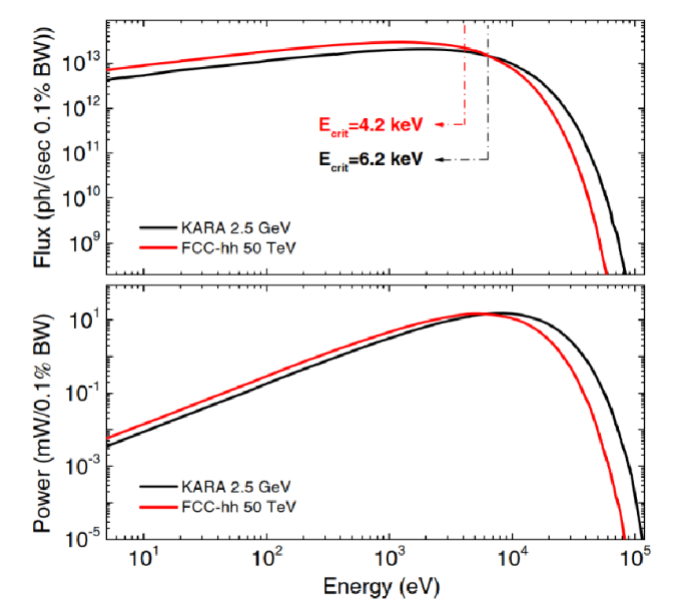
\includegraphics[width=\textwidth]{graphics/wp3-KIT_FCCphotons.png}
  \end{minipage}%
  \hfill
  \begin{minipage}[c]{0.5\textwidth}
    \vspace*{\fill}
    \captionof{figure}{Comparison of the photon flux (top) and power (below) of the FCC-hh at \SI{50}{TeV} proton beam energy in comparison with KARA's at its nominal \SI{2.5}{GeV} electron energy for user %operation. Calculations were performed with SYNRAD+~\footnote{see: L. A. González et al. DOI: 10.1103/Phys.Rev.Accel.Beams 22, 083201, and L. A. González et al. (2021) Phys.Rev.Accel.Beams 24, 113201}
    }
    \label{fig:yourlabel}
    \vspace*{\fill}
  \end{minipage}
\end{figure}

During the EU-project EuroCirCol CERN and KIT realized the BESTEX beamline of CERN at the KIT light source. The storage ring of the KIT light Source is the synchrotron KARA delivering similar spectra as expected at the FCC.

CERN installed a residual gas analyser in the central part of the BESTEX test chamber  before the start of the FCC beam screen prototype experiment (no.5, with saw-tooth profile to decrease synchrotron radiation photon scattering) in period P1 (EURO-LABS-KIT-KARA-2023-01). In period P2 this prototype was exchanged by the new beam-screen prototype no. 6 with amorphous carbon coating (aC). aC is a stable and inert material, deposited via sputtering techniques onto the internal wall of a circular tube (carried out at CERN).  The main feature of aC is its extremely low secondary electron yield, which is necessary to avoid electron cloud instability in accelerators with positively charged beams. In the long-term experiment at KARA (EURO-LABS-KIT-KARA-2023-03), the beam-screen prototype no. 6 was irradiated at a flat angle of incidence and cooled with LN2. The increase in pressure was measured. In addition, the composition of the species outgassing from the beam screen was determined at CERN's BESTEX beamline at KARA. The experiment began installation in August 2023 and the prototype was irradiated with over 480 KARA synchrotron light until the first quarter of 2024. The prototype is still installed in BESTEX and is waiting to be exchanged for the next one, which is currently being prepared
\begin{figure}[!h]
    \centering
    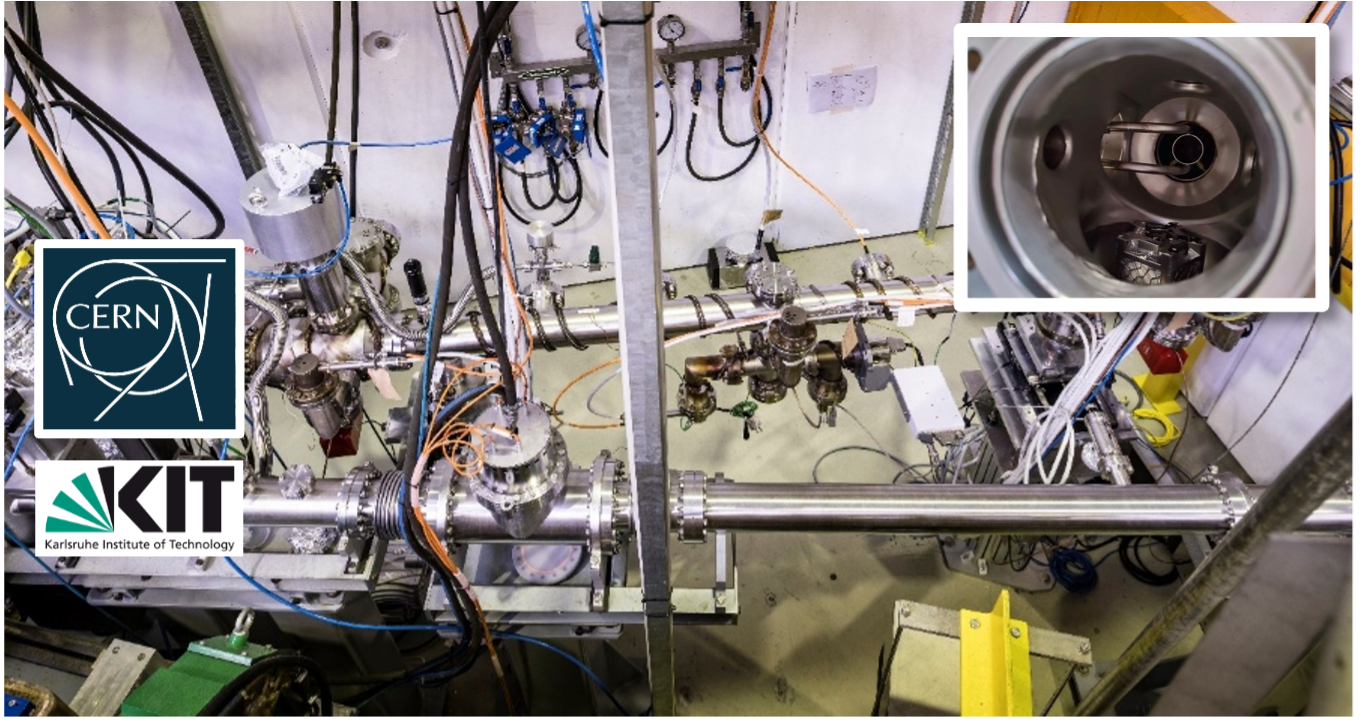
\includegraphics[width=0.75\linewidth]{graphics/wp3-KIT_BESTEX.png}
    \caption{CERN installed the BESTEX beamline at KARA since 2019 (EU project EuroCirCol). BESTEX was used for up to now two actual TA experiments within EURO-LABS. A goal is the exploration of the vacuum performance of the FCC-hh beam screen to protect the cold superconducting magnets from the 
direct irradiation high-power SR photon beams.
}    
    \label{fig:kit_bestex}
\end{figure}

The KARA experiment (EURO-LABS-KIT-KARA-2023-04) of the University Lille aimed to observe, understand and control the ultrafast self-organisation of relativistic electron bunches in accelerator facilities. A central goal is to master the emission of giant terahertz (THz) pulses in coherent synchrotron radiation (CSR), which is a proposal for new THz sources. Another important goal was the improvement of novel ultrafast observation instruments. KARA is one of the only electron storage rings in the world where the shape of relativistic electron bunches can be directly ‘studied’ in a storage ring facility. The techniques of chaos control (feedback control of periodic orbits) for achieving stable THz-CSR emissions, which the team at the University of Lille had already successfully tested at the SOLEIL synchrotron, were transferred to the KIT light source KARA, and the results have thus been compared between the machines and with theory. At KARA, the opportunity was taken to observe the development of the longitudinal bunch profile in real time with the help of the existing electro-optical near-field setup. In this experiment, an advanced control loop from chaos control theory was implemented on a fast FPGA board to control the amplitude of one of the two main radiofrequency (RF) cavities in the electron storage ring KARA at KIT. The CSR emission of THz power at high level was stabilised to control the micro-bunching instability. The fast Schottky diodes in the KIT-IR2 beamline at KARA were used and the THz power was measured in real time with the high-speed data acquisition card KAPTURE developed by KIT.
\begin{figure}[H]
    \centering
    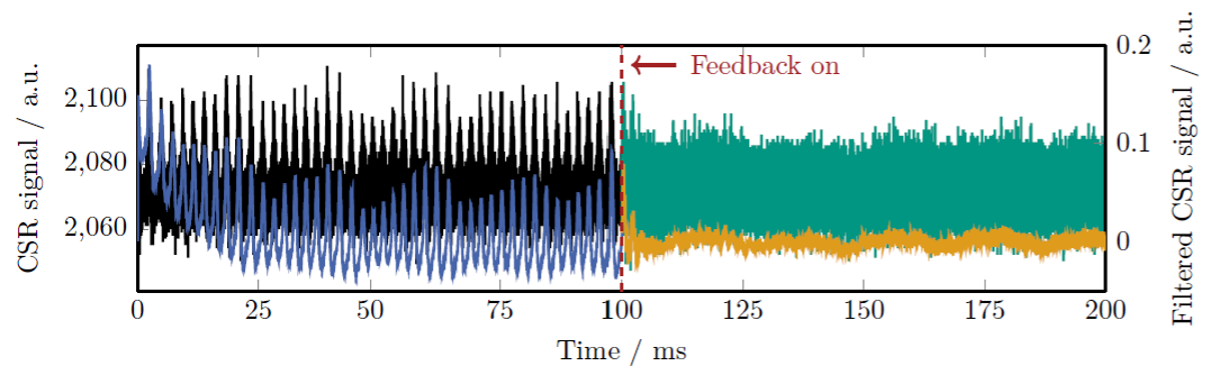
\includegraphics[width=0.75\linewidth]{graphics/wp3-KIT_CSRsignal.png}
    \caption{The CSR signal was measured with a fast Schottky diode (at a KIT infrared beam line). After \SI{100}{ms} the team of the University Lille (F) switched on the FPGA-based feedback loop. For better visibility, the raw signal (black, left \& green, right) was filtered (blue, left \& orange, right) to remove the fast sinusoidal fluctuation. Suppression of the sawtooth outburst fluctuation variance by a factor of 28 in the CSR emission at the KARA electron storage ring, after switching on the FPGA-based feedback loop developed by the PhLAM team of University Lille. The fast CSR fluctuations are still present after the feedback is switched on, leading to a stabilization of the THz emission. Publication in preparation.}    
    \label{fig:kit_csr}
\end{figure}

FCC-ee precision physics measurements require an accurate and precise determination of the centre-of-mass collision energy, which can be obtained from the beam energies. Since the depolarisation frequency is directly proportional to the beam energy, a promising way to determine this energy is to depolarise transversely polarised packets. This resonant depolarisation (RDP) has long been used in KARA whereby the resonance frequency is measured via the change in the Touschek lifetime. At KARA, a first RDP measurement campaign (EURO-LABS-KIT-KARA-2023-05) with numerous scan settings and bundle configurations was carried out to investigate how this technique could be applied at FCC-ee, in particular the sensitivity to parameters such as the scan speed of the depolariser and the scan velocity. The measurement campaign was successful and the users at CERN expressed interest in carrying out another measurement campaign at a later target point.
\begin{figure}[H]
    \centering
    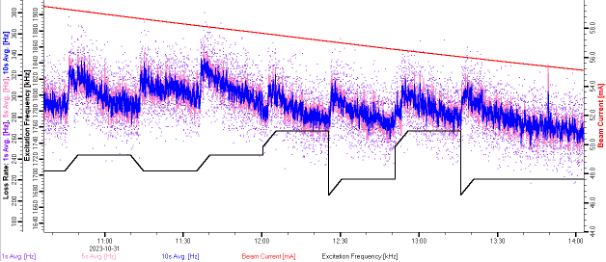
\includegraphics[width=0.75\linewidth]{graphics/wp3-KIT_RDPscans.png}
    \caption{More than 40 successful RDP scans were realized at KARA by scanning direction up and down for scanning times of \SI{100}{s} to \SI{600}{s}, respectively}    
    \label{fig:kit_rdp}
\end{figure}

RDP results published in:
\begin{itemize}
\item FCCIS WP2-workshop, 2023-11-15, B. Härer et al.: Polarisation studies at KARA
\item and in the following IPAC papers: \\ https://doi.org/10.18429/JACoW-IPAC2024-TUPG33, \\ https://doi.org/10.18429/JACoW-IPAC2024-WEPG51, and \\ https://doi.org/10.18429/JACoW-IPAC2024-WEPR20
\end{itemize}

Bunch-by-bunch (BBB) feedback systems are essential for the realisation of ultra-low emittance rings that allow electron beams to reach high-quality states for use in synchrotron radiation light sources and colliders. Following the workshop WP7.2 of the EU project I.FAST on BBB feedback systems, which was attended by more than 40 experts on BBB systems from all over the world, the following three experiments were carried out at the request of the experts in connection with the BBB systems carried out at the KARA storage ring and at the booster synchrotron with real electron beams by operating the BBB systems installed in each of the two accelerators(EURO-LABS-KIT-KARA-2024-06). The aim of the first experiment at KARA was to manipulate the vertical beam size by exciting the betatron oscillation with the BBB system to improve the Touschek beam lifetime. The goal of this experiment was to look for common procedures for commissioning bunch-by-bunch feedback systems. The goal of the third experiment was to longitudinal kicks with the bunch-by-bunch feedback system and the stripline kicker installed in the booster synchrotron. This experiment will lead to the next step, such as longitudinal manipulation of beams to improve booster beam quality. Data and results of the three experimental topics have been shared with all interested participants, and the data analysis and subsequent discussions are ongoing. 
\begin{figure}[H]
    \centering
    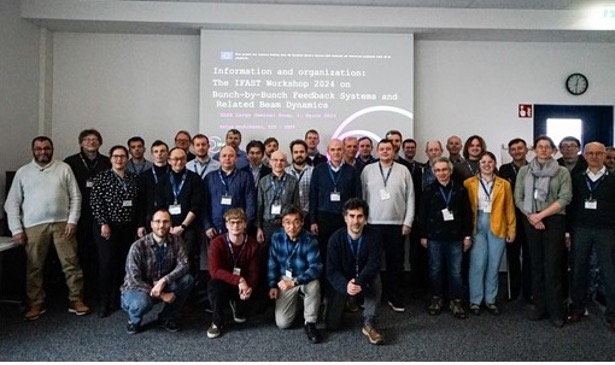
\includegraphics[width=0.75\linewidth]{graphics/wp3-KIT_iFASTevent.jpg}
    \caption{Joint experimental campaign 5th – 6th March 2024 with 29 onsite users at KIT following the I.FAST workshop on BBB feedback systems. TA within EURO-LABS, WP 3.3  and  Networking within I.FAST, WP 7.2: https://indico.scc.kit.edu/event/3742/
Three experiments were defined by the users and carried out: vertical emittance / beam size control with BBB feedback system; search for a common way to commission BBB feedback systems; test for modulation the longitudinal motion of the KARA booster synchrotron beam with a strip-line kicker.}    
    \label{fig:kit_ifast}
\end{figure}

According to the design of the FCC, the desired mechanical alignment tolerances of the magnets are in the range of \SI{100}{\micro\meter} to \SI{150}{\micro\meter}. However, to achieve the ambitious research goals at the FCC, a low (10-20 µm) relative alignment of the quadrupoles and sextupoles is required. For this purpose, correction magnets are provided to steer the beam in the direction of the magnetic centre, which is known as beam-based alignment (BBA). The BBA must be performed for approx. 1870 quadrupoles and approx. 630 sextupoles, so in addition to the accuracy, the average time required to determine the individual magnetic offset is a key parameter for the selection of the BBA method. The development of a concept for the BBA at FCC-ee is currently based on simulations but is to be supported by proof-of-principle tests on existing machines, for which experiments were carried out at KARA (EURO-LABS-KIT-2024-KARA-07).  Strategies were successfully investigated that will significantly reduce the time required for the BBA at FCC.

On the \textbf{TA marketing:}

At each conference in which we present an overview of our accelerator facilities ALFA = KARA and FLUTE, KIT draws attention to the Transnational Access (TA) offer as part of the EU funding in the EURO-LABS project. On KIT websites implementation of the marketing for Transnational Access (TA) promised in the EURO-LABS application with partial funding within the framework of the EU project EURO-LABS on our following Internet pages:
\begin{itemize}
\item https://www.ibpt.kit.edu/alfa.php, among the films that were (partially) funded by EURO-LABS

\item https://www.ibpt.kit.edu/user.php, under the 4 points on ‘Proposal Submission System
\end{itemize}

On the \textbf{Service Improvements:}

\underline{\em{Simulation and Measurement Framework activities}}: \\ 
The frame work online optics simulation in ocelot was extended by scripts to measure automated different accelerator parameters like chromaticity, dispersion, beta function and response matrix. Further tools for different beam bases alignment  techniques are currently in development together with one TNA activity. Another class of measurements are camera image processing. There different open source tools and analysis frameworks have been evaluated. It was decided to use the area Detecot (Ref: https://areadetector.github.io/areaDetector/index.html) for this application which is currently implemented at KARA and FLUTE. KIT also joined the python accelerator middle layer activities (Ref: https://github.com/python-accelerator-middle-layer) to benefit from the shared effort. The next step is to contribute to the code development and deployment of the system at KARA and FLUTE.

\underline{\em{Data Management Framework Activities}}: \\ 
In-depth analysis and comparison of three research data management platforms: B2Share~\footnote{https://b2share.eudat.eu/}, RADAR~\footnote{https://radar.products.fiz-karlsruhe.de/en}, and Kadi4Mat~\footnote{https://kadi.iam.kit.edu/}. This evaluation aimed to select suitable tools for managing experimental physics data effectively. Each platform was assessed based on its capabilities for data storage, accessibility, and metadata handling. Special attention was given to the ability to structure and retrieve metadata efficiently. Analyzing different experiments revealed that the metadata must be identified at an individual measurement level. This ensures precise documentation and supports reproducibility in research workflows. A flexible metadata generation schema is under preparation to accommodate diverse experimental requirements. The evaluation also considered automation possibilities to reduce manual metadata entry. Security, scalability, and integration with existing infrastructure were additional factors in the assessment. The final selection will balance usability and long-term sustainability for research environments.

Next steps: Based on the gained experience, select the most suitable tool and implement the Data Handling Framework and metadata generation. Validate the chosen solution in real-world scenarios and refine the approach based on feedback.

\separatorline{0.3em}{0.5\textwidth}{0.4pt}

\subparagraph{CLARA}
 
During the reporting period, the CLARA facility has continued its reconfiguration to enable operation at \SI{250]{MeV}. In parallel, the full energy beam exploitation (FEBE) experimental hutch has been assembled and major sub-assemblies such as the user experiment chambers, magnetics and light boxes have been installed. The FEBE Ti:sapphire laser system has also been commissioned, allowing the synchronised interaction of electron bunches with a $\sim$\SI{100}{TW} laser.
 
As of March 2025, the CLARA build phase is complete and the electron gun has been successfully tested. Due to the extensive redevelopment of CLARA and delays to the operational reinstatement of the facility, the facility has not delivered any TA projects during the period. However, sub-system recommissioning and beam threading will continue through summer 2025 and it is anticipated that user beam access, including TA projects, will restart in Q3/Q4 2025.

\separatorline{0.3em}{0.5\textwidth}{0.4pt}

\subparagraph{LPA UHI100 (CEA-LIDYL} No beamtime delivered during P2 (as well as P1) due to a delay induced by the delay of the  French Nuclear Safety Authority (ASN) to deliver a license for operating the facility. We are still waiting for the final license from the ASN / CEA.

We have moved our whole experimental facility (laser and experimental equipments) from the main CEA site (Saclay) to a satellite one (Orme des Merisiers), few kilometers away. Before being authorized to shoot full laser energy on target to deliver the laser driven electron source, we had to ask for a license from ASN (Nuclear Safety Authority). A first temporary one was delivered from the beginning of 2024 up to the end of august 2024, limiting the generating conditions to \SI{50}{MeV} maximum electron energy, 1 shot per minute and a maximum of 15pC/bunch, which means degraded generating conditions. A visit from ASN has been scheduled last July 3rd, 2024, to assess the operating conditions at our laboratory. During this visit, we received feedback regarding modifications, and we have submitted a revised request for experimental parameters in line with our scientific program (higher energy, repetition rate and charge in the electron beams).
An authorization from ASN was sent to CEA at the end of December 2024 for communication on January 13th to our team. This is a temporary license valid for one year, with the following parameters: 200 MeV, a maximum repetition rate of 0.3 Hz, and a maximum charge of 300 pC/bunch.
Before conducting full-power operations on target, we need to perform test experiments (initial regulatory check to record the dose deposited by electrons and check the consistency of simulations and experiments. These tests are planned next March 2025, and once completed, if everything is consistent, we should be able to proceed with full-power operations on target.

\subsubsection*{Deviations and Corrective Actions}

\todo{Briefly summarise any deviations and performed corrective actions of the WP in context of the DoA.}

\subparagraph{LPA UHI100 (CEA-LIDYL)} We have plan to deliver beamtime as much as we will be able to do. We have already a proposal from an Italian Team that should be submitted. The LPA-UHI100 facility team is considering the technical feasibility of the proposal with the applicants, before submission. And we are working on a 2nd proposal which could be the following of the 1st one, depending on the results obtained. We will keep advertising about the TNA through EUROLABS, participating to international/national conferences this year 2025.  We have already discussed with other communities and in particular physico –chemists and radiobiologists who want to use the extrem dose rate delivered by our laser-driven electron sources to test the response of biological material to such irradiations, in the context of FLASH radiotherapy, and to validate dosimeters developed for such high dose rate source.  


1 beam time project (160 hours)for this year , in preparation for submission next march 2025, to test a temporal diagnostic adapted to the extremely short duration of the LPA electron beams. The beamtime could be allocated at the second semester 2025.

We will try to deliver another beamtime period (160hours) in the first semester 2026, planning a maximum of 2 runs in 2026 (320hours max in 2026).

\subparagraph{LNF facilities perspectives till the EUROLABS conclusion}

The perspectives for the completion of the EUROLABS TA program for BTF look quite secure. The facility staff is now systematically promoting the opportunity of supported TA to the reference community, with positive returns, and 4 out of 7 TA weeks planned for the whole project have been already delivered. The staff is confident that the remaining 3 will be assigned and delivered by the end of 2025, and some space will be available to eventually accommodate 2-3 extra weeks in the 2026 before the project conclusion.
For what concerns SPARCLAB the situation looks far less optimal. As mentioned, none of the 9 weeks of TA allocated in the project have been delivered so far, and it not realistic to think recovering all in the time left till the end of the project for the mentioned reasons. In 2025 the new facility EuAPS funded by the Next Generation EU program will be installed in the SPARCLAB bunker requiring a 4 months shutdown. In the present scenario the number of allocable TA weeks at SPARCLAB before the EUROLABS project end in August 2026 is 2-3. The SPARCLAB staff is committed to promoting this opportunity to its international reference community.


\subparagraph{Task 3.4 : Applications} \mbox{}

% \todo{Briefly explain the progress of the task in context to the DoA.}


Task 3.4 includes two facilities: the {\bf INCT/RAPID} and the {\bf CERN/CLEAR}.

During the reference period both facilities were able to deliver a sizeabl amount of Transnational Access to a variety of projects. Details are briefly described below. 

\subsubsection*{Main Results and Achievements}

% \todo{Briefly summarise the main results and achievements of the WP in context of the DoA.}

\subparagraph*{INCT RAPID Facility} In the reporting period 2 INCT Rapid infrastructure provided access with EURO-LABS support carrying out 7 projects (one projects is still ongoing). The experiments were carried using the following instruments: 
\begin{itemize}
\item LAE 10 accelerator with nanosecond pulse radiolysis sat-up – to investigate basic mechanisms of ionising radiation interactions in biological systems.
\item Electronica accelerator, generating beam of electrons of energy 10 MeV – for sterilization and materials modification
\item ILU 6 accelerator, using electron beam of energy 1.7 MeV and energies < 300 keV – for controlled depth of electron range in treated products.
\end{itemize}
For the experiments carried out at RPAID infrastructure the dosimetry measurements were performed by INCT Labotartru of Technological Dose Measurements, to ensure precise and accurate dose delivery in treated samples. Also additional INCT infrastructure supported carried out experiments was used, e.g Electron Paramagnetic Spectroscopy to help characterise radiation induced effects in materials.

The experiments were focused on application of electron beam to investigate the mechanisms of radicals interactions, radiation induced effects in materials and effects of electron beam irradiation on food and food ingredients: 
\begin{itemize}
\item One-electron oxidation of S-adenosyl methionine,
\item Crosslinking of self-assembled fatty acids on copper by electron beam irradiation,
\item Effect of ionizing irradiation on dried fruits,
\item Influence of 10 MeV accelerated electrons on structure and properties of sheep wool fibres as a potential component for preparation of polymer-based composite materials
\item Irradiation engineering of biopolymer-based formulation for wound management and targeted drug delivery devices,
\item Bioactivity of irradiated foods by low energy e-beam,
\item Face masks recycling with the use of radiation technologies.
\end{itemize}
In the upcoming year it is planned to adjust experimental set-up for irradiation in gaseous phase, as a response to newly received project request. This will broaden the area of research carried out at INCT within EURO-LABS.

\separatorline{0.3em}{0.5\textwidth}{0.4pt}

\subparagraph*{CERN-CLEAR Facility}

CLEAR delivered TA to four projects during the reference period. 
\begin{description}
    \item[AI1] Artificial Intelligence readiness at CLEAR. Done, Reimbursed (A. Pollastro, 40 units)
    \item[LUXE2] Done, reimbursed (F. Lasagni-Manghi, 40 units)
    \item[THz] THz sources on Smith-Purcell radiation, THZ1 > Initial visit + preparation done, 
will not be reimbursed (paid by Users Lab) (T. Zhang, 16 units)
    \item[SE1] Electron collimation at CLEAR (SE1) > Done, to be reimb. (N. Delerue, D. Dauvergne, 64 units)
\end{description}

On the \textbf{Service Improvements:}

\todo{good progress - waiting some text from Roberto}

\subsubsection*{Deviations and Corrective Actions}

\todo{Briefly summarize any deviations and performed corrective actions of the WP in context of the DoA.}

\subsubsection*{Milestones and Deliverables}

%{\fontsize{9}{11}\selectfont
%\begin{center}
%  \begin{tabular}[t]{!{\color{mygray}\vrule}p{0.10\linewidth}!
%  {\color{mygray}\vrule}p{0.60\linewidth}!
%  {\color{mygray}\vrule}p{0.20\linewidth}!{\color{mygray}\vrule} } \hline
%    \rowcolor{mycyan} & {\bf Title} & {\bf Status} \\ \hline
%    \cellcolor{mycyan}{\bf D1.x}: &  &  \\ \hline
%  \end{tabular}
%\end{center}
%}

There were no Milestones nor Deliverables for WP3 for the reference period. 

\subsubsection*{Project Meetings}

%  {\color{mygray}\vrule}p{0.40\linewidth}!

%%%%%%%%%%%%%%%%%%%%%%%%%%%%%%%%%%%%%%%%%